% 按 1991 全国文科原页重绘点线连接关系；投影仅示意，不表示比例。
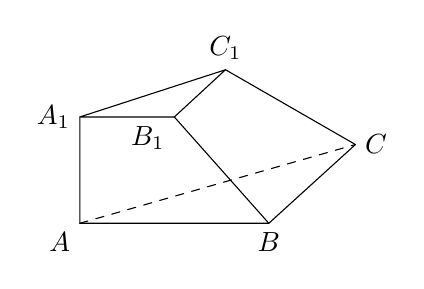
\begin{tikzpicture}[line join=round,line cap=round]
  \coordinate (A)  at (0,0);
  \coordinate (B)  at (2.4,0);
  \coordinate (C)  at (3.5,1.0);
  \coordinate (A1) at (0,1.35);
  \coordinate (B1) at (1.2,1.35);
  \coordinate (C1) at (1.85,1.95);
  \draw (A)--(B)--(C);
  \draw[dashed] (A)--(C);
  \draw (A)--(A1) (B)--(B1) (C)--(C1);
  \draw (A1)--(B1)--(C1)--cycle;
  \node[below left]  at (A)  {$A$};
  \node[below]       at (B)  {$B$};
  \node[right]       at (C)  {$C$};
  \node[left]        at (A1) {$A_1$};
  \node[below left]  at (B1) {$B_1$};
  \node[above]       at (C1) {$C_1$};
\end{tikzpicture}
